\documentclass[12pt]{article}

\usepackage[utf8]{inputenc}
\usepackage[T1]{fontenc}
\usepackage{a4}
\usepackage{lipsum}
\usepackage{graphicx}
\usepackage{float}
\usepackage{listings}
\usepackage{color}
\usepackage{cite}
\usepackage{textgreek}
\usepackage{amsfonts}

\usepackage[margin=1in]{geometry}

\definecolor{dkgreen}{rgb}{0,0.6,0}
\definecolor{gray}{rgb}{0.5,0.5,0.5}
\definecolor{mauve}{rgb}{0.58,0,0.82}

\lstset{frame=tb,
  language=matlab,
  aboveskip=5mm,
  belowskip=5mm,
  showstringspaces=false,
  columns=flexible,
  basicstyle={\small\ttfamily},
  numberstyle=\tiny\color{gray},
  keywordstyle=\color{blue},
  commentstyle=\color{dkgreen},
  stringstyle=\color{mauve},
  breaklines=true,
  breakatwhitespace=true,
  tabsize=2
}

\title{
  {\Huge \bf Power Systems Lab}\\
  \vspace{0.25in}

  {\bf Experiment 1}\\
  Laboratory Report
  \vspace{1in}
}
\author{
  \bf Syed Alisamar Husain, 17BEE012\\
  B.Tech Electrical Engg, 8th Semester
}

\begin{document}
  \begin{titlepage}
    \maketitle
    \vspace*{\fill}
    \begin{center}
      {\bfseries Department of Electrical Engineering} \\
      Jamia Millia Islamia, New Delhi
    \end{center}
    \thispagestyle{empty}
  \end{titlepage}
  
  \newpage
  \begin{center}
    \huge Experiment 1
    \vspace{0.5in}
  \end{center}

  \section{Objective}
  To evaluate the equivalent pi-model and the transmission matrix 
  for a 3-phase long transmission line.

  {\bf Let the given problem be as follows:}
  \begin{center}
    \itshape
    A 3-phase, 60 Hz, completely transposed, 345 kV, 200 km long line
    has two ACSR conductors per bundle and the following constants,\\
    Impedance (Z) =  0.017 + j 0.12 $\Omega$ / km\\
    Admittance (Y) = j 1.2 $\times 10^{-6}$ $S$ / km\\
    Find the transmission matrix using the equivalent pi-model.
  \end{center}

  \section{Theoretical Background}
  {\bf A long transmission line} is defined formally as a power transmission 
  line with an effective {\bf length more than 250 km} (150 miles). 
  Unlike short transmission lines and medium transmission lines, 
  it is no longer reasonable to assume that the line parameters 
  are lumped. To accurately model a long transmission line we 
  must consider the exact effect of the distributed parameters 
  over the entire length of the line. 
  
  Although this makes the calculation of ABCD parameters of 
  transmission line more complex, it also allows us to derive 
  expressions for the voltage and current at any point along the line.

  {\bf In a long transmission line the line constants are uniformly 
  distributed over the entire length of line.} This is because the 
  effective circuit length is much higher than what it was for the 
  former models (long and medium line) and hence we can no longer 
  make the following approximations:
    \begin{itemize}
      \item {\bf We cannot ignore the shunt admittance} of the network, 
      like in a small transmission line model.
      \item Considering the circuit {\bf impedance and admittance to be 
      lumped} and concentrated at a point as was the case for the 
      medium line model.
    \end{itemize}

    \pagebreak
    \subsection{The Nominal $\pi$-model}
    In the Nominal $\pi$ Model, the shunt capacitance of each line i.e. 
    phase to neutral is divided into two equal parts. 

    \begin{figure}[H]
      \begin{center}
        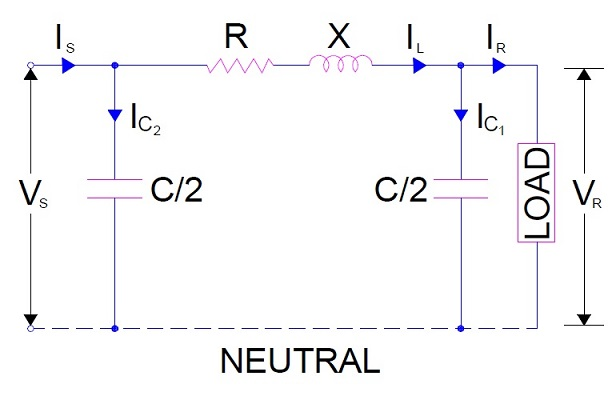
\includegraphics[width=3in]{img/Nominal-pi-method.jpg}
        \caption{Nominal $\pi$-Model}
        \label{nominal-pi}
      \end{center}
    \end{figure}

    One part is lumped at the sending end while the other is lumped at 
    receiving end as shown in Figure \ref{nominal-pi}.

    \subsection{The Equivalent $\pi$-model}
    \begin{figure}[H]
      \begin{center}
        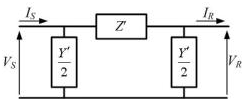
\includegraphics[width=3in]{img/eqv-pi.png}
        \caption{Equivalent $\pi$-Model}
      \end{center}
    \end{figure}
    The equivalent $\pi$-model does not make the assumption that the 
    impedance and admittance of the line is lumped at the ends like in the
    case of a short or medium transmission line.
    This model takes into account that the impedance and admittance of the line
    is distributed along the line.

  \pagebreak
  \section{Implementation}
  \begin{lstlisting}
    % Equivalent pi-model and the transmission matrix

    Zp  = 0.017 + 0.12i; % Impedance per km
    Yp  = 1.2i;          % Admittance per km
    len = 200;           % Length in km

    Z = len * Zp;   % Total Impedance
    Y = len * Yp;   % Total Admittance

    A = ((Y*Z)/2) + 1;
    B = Z;
    C = Y*(((Y*Z)/4) + 1);
    D = A;

    T = [ A B; C D; ]
  \end{lstlisting}

  \section{Observations}
  \begin{figure}[H]
    \begin{center}
      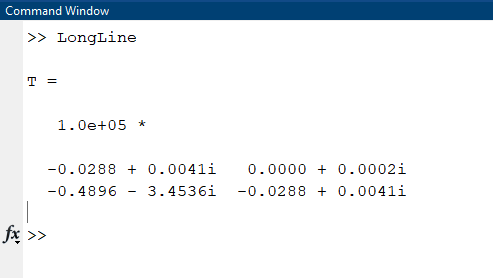
\includegraphics[width=4in]{img/result.png}
      \caption{Result}
      \label{result}
    \end{center}
  \end{figure}
  The result of the above program with the given parameters 
  is shown in figure \ref{result}.


  \section{Result}
  We calculated the transmission matrix (i.e. ABCD parameters) of the long
  transmission line using the Equivalent $\pi$-Model method in MATLAB.

\end{document}